\documentclass[final]{beamer}

% Use beamerposter with A0 portrait
% \usepackage[size=a0,orientation=landscape,scale=1.05]{beamerposter}
\usepackage[size=a0,orientation=portrait,scale=1.05]{beamerposter}

% Basic packages
\usepackage[utf8]{inputenc}
\usepackage[T1]{fontenc}
\usepackage{lmodern}
\usepackage{graphicx}
\usepackage{booktabs}
\usepackage{multicol}
\usepackage{wrapfig}
\usepackage{natbib}
\bibliographystyle{unsrtnat}

% \usepackage{enumitem} % REMOVED to avoid beamer conflict
\usepackage{hyperref}
\usepackage{array}
\usepackage{ragged2e}
\usepackage{colortbl}
\usepackage{xcolor}
\usepackage{etoolbox} % for safe list tweaks

% Safer list spacing
\makeatletter
\patchcmd{\itemize}{\def\makelabel}{\setlength{\itemsep}{0.4em}\def\makelabel}{}{}%
\patchcmd{\enumerate}{\def\makelabel}{\setlength{\itemsep}{0.4em}\def\makelabel}{}{}%
\makeatother

% Colors
\definecolor{royal}{HTML}{2C3E50}
\definecolor{accent}{HTML}{4A90E2}
\definecolor{softbg}{HTML}{F8F7F4}
\definecolor{danger}{HTML}{C0392B}

\setbeamercolor{normal text}{fg=royal,bg=softbg}
\setbeamercolor{block title}{fg=white,bg=accent}
\setbeamercolor{block body}{fg=royal,bg=white}
\setbeamercolor{alerted text}{fg=danger}
\setbeamercolor{structure}{fg=accent}

\usefonttheme{professionalfonts}
\setlength{\parskip}{0.6em}
\setlength{\parindent}{0pt}
\newcommand{\key}[1]{\textbf{\color{accent}#1}}

% Paper size
% \setlength{\paperwidth}{841mm}
% \setlength{\paperheight}{1189mm}

\title{\LARGE \textbf{Refining the Sunspot Number Series to ISN~V3:\\ Challenges and Benefits for the Space Climate Community}}
\author{\large Kalugodu Chandrashekhar$^{1}$, Laure Lef\`evre$^{1}$, Benjamin Mampaey$^{1}$, Senthamizh Pavai Valliappan$^{1}$, Hisashi Hayakawa$^{2}$, Christian Ritter$^{3}$}
\institute{\large $^{1}$ Royal Observatory of Belgium (ROB), $^{2}$ Nagoya University, $^{3}$ Universit\'e Catholique de Louvain, Louvain-la-Neuve, Belgium}

% Logos (replace with your own files)
\newcommand{\leftlogo}{./logos/observatory_400x332.jpg}
\newcommand{\rightlogo}{./logos/BELSPO_1867x1563.jpg}

% Title box
\setbeamertemplate{headline}{%
  \leavevmode%
  \begin{beamercolorbox}[wd=\paperwidth,ht=5.2cm]{block body}
    \begin{minipage}[c]{0.19\paperwidth}
      \centering \vspace{0.6cm}
      \includegraphics[height=3.6cm]{\leftlogo}
    \end{minipage}%
    \begin{minipage}[c]{0.62\paperwidth}
      \centering \vspace{0.4cm}
%      {\color{royal}\bfseries\fontsize{73}{76}\selectfont FAR\textcolor{accent}{Su}N}\\[0.4cm]
      {\color{royal}\bfseries\fontsize{36}{40}\selectfont \inserttitle}\\[0.3cm]
      {\large \insertauthor}\\[-0.2cm]
      {\normalsize \insertinstitute}
    \end{minipage}%
    \begin{minipage}[c]{0.19\paperwidth}
      \centering \vspace{0.6cm}
      \includegraphics[height=3.6cm]{\rightlogo}
    \end{minipage}
  \end{beamercolorbox}%
}

% Footer
\setbeamertemplate{footline}{%
  \begin{beamercolorbox}[wd=\paperwidth,ht=1.2cm]{block body}
    \hfill \small \textbf{Contact:} your.email@institution \quad|\quad \textbf{Project:} \url{https://www.sidc.be/silso/} \hfill
  \end{beamercolorbox}%
}

% Helper block env
\newenvironment{tightblock}[1]{%
  \begin{block}{#1}\vspace{-0.5em}
}{\end{block}}

\begin{document}
\begin{frame}[t]
\begin{columns}[t,totalwidth=\paperwidth]

% -------- COLUMN 1 --------
\begin{column}{0.32\paperwidth}
\begin{tightblock}{Abstract}
\justifying
The International Sunspot Number (ISN) series, a cornerstone for space climate studies, still exhibits scale discrepancies despite recent recalibrations, underscoring the critical need for a comprehensive reconstruction from raw historical observations. The FARSuN (Findability and Accessibility of historical Raw Sunspot Numbers) project addresses this by systematically gathering, digitizing, and standardizing scattered sunspot data from 1607-1980, aiming to bridge the technical and scientific gap preventing holistic data use. Significant progress includes the digitization of Prof. Wolf's Mittheilungen (1610-1918) and the near-completion (95\%) of more than 2000 Zürich observation tables, transforming them into machine-readable formats. Data extractions for challenging sources like Gruithuisen, Stark, Adams, and Rost are actively underway, supported by advanced tools like Transkribus and rigorous quality control efforts to define homogeneous metadata criteria. Upcoming initiatives include a citizen science web interface to engage the public in data recovery and the ultimate goal of constructing a new, consolidated ISN (V3) and historical hemispheric sunspot numbers. This comprehensive reconstruction will provide the Space Climate Community with an unprecedentedly accurate and accessible record, significantly improving solar cycle predictions, understanding long-term solar variability, space weather discussions, and refining climate models.
\end{tightblock}

\begin{tightblock}{Why Reconstruction?}
  The International Sunspot Number (ISN) suffers from historical inconsistencies, like the "Waldmeier jump" around 1947. Previous attempts to fix this were limited to *recalibration*. FARSuN's approach, a full **reconstruction**, is fundamentally different and more robust.
\begin{itemize}
  \item Recalibration adjusts an existing index, biases may persist.
  \item Reconstruction returns to primary sources (Historical journals, drawings, manuscripts, tables).
  \item Tackles observer-dependent scale changes (“Waldmeier jump” from \cite{svalgaard2013}) .
\end{itemize}
\end{tightblock}

\begin{tightblock}{Four-Axis Methodology}
\begin{enumerate}
  \item \key{Gather Sources} : archives, manuscripts, tables (Identify and locate historical sunspot data)
  \item \key{Process Data} : digitize, OCR/HWR, Transkribus (Extract and normalize data)
  \item \key{Validate \& Standardize} : homogeneous metadata for scientific usability
  \item \key{Disseminate} : FAIR principles, VO-ready access
\end{enumerate}
\end{tightblock}

\begin{tightblock}{FAIR Principles}
  The project ensures FAIR (Findable, Accessible, Interoperable, Reusable) principles, making the final dataset robust and accessible for future science.

\begin{itemize}
  \item \textbf{Findable} – DOIs, metadata
  \item \textbf{Accessible} – open formats
  \item \textbf{Interoperable} – vocabularies, VO compliance
  \item \textbf{Reusable} – versioning, uncertainties
\end{itemize}
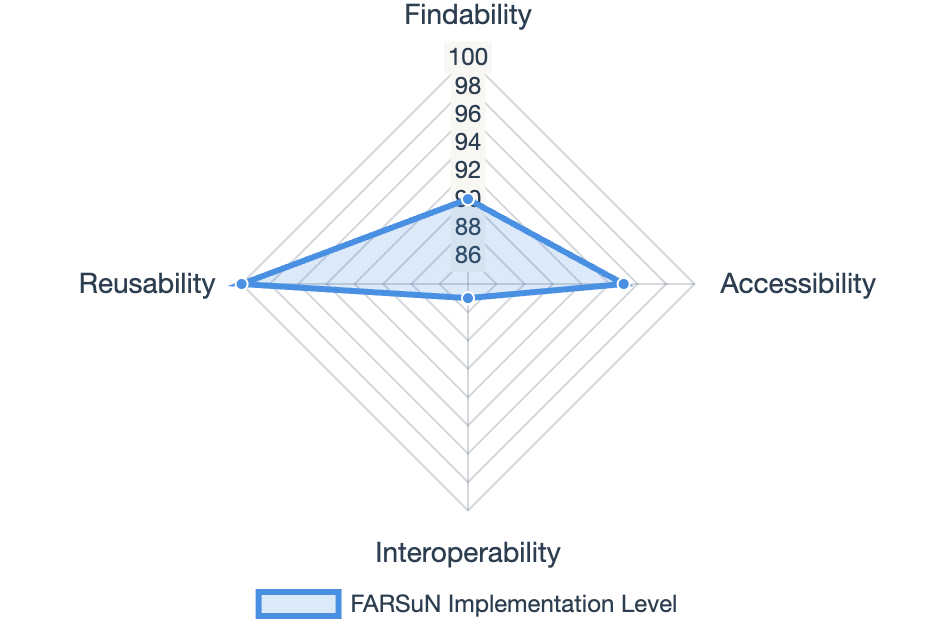
\includegraphics[width=\linewidth]{./figures/fair_radar.png}
\end{tightblock}
\end{column}

% -------- COLUMN 2 --------
\begin{column}{0.32\paperwidth}
\begin{tightblock}{Key Datasets}
\begin{tabular}{@{}p{0.35\linewidth}p{0.2\linewidth}p{0.4\linewidth}@{}}
\toprule
\textbf{Source} & \textbf{Period} & \textbf{Status} \\ \midrule
Zürich Tables & 1945–1979 & 95\% digitized \\
Mittheilungen & 1610–1918 & Integrated indices \\
Gruithuisen & 1800s & In progress (Kurrent) \\
Adams & 19–20c & Drawings under extraction \\
Stark & 18–19c & Tabular records \\
Rost & 18–19c & Metadata normalization \\
\bottomrule
\end{tabular}
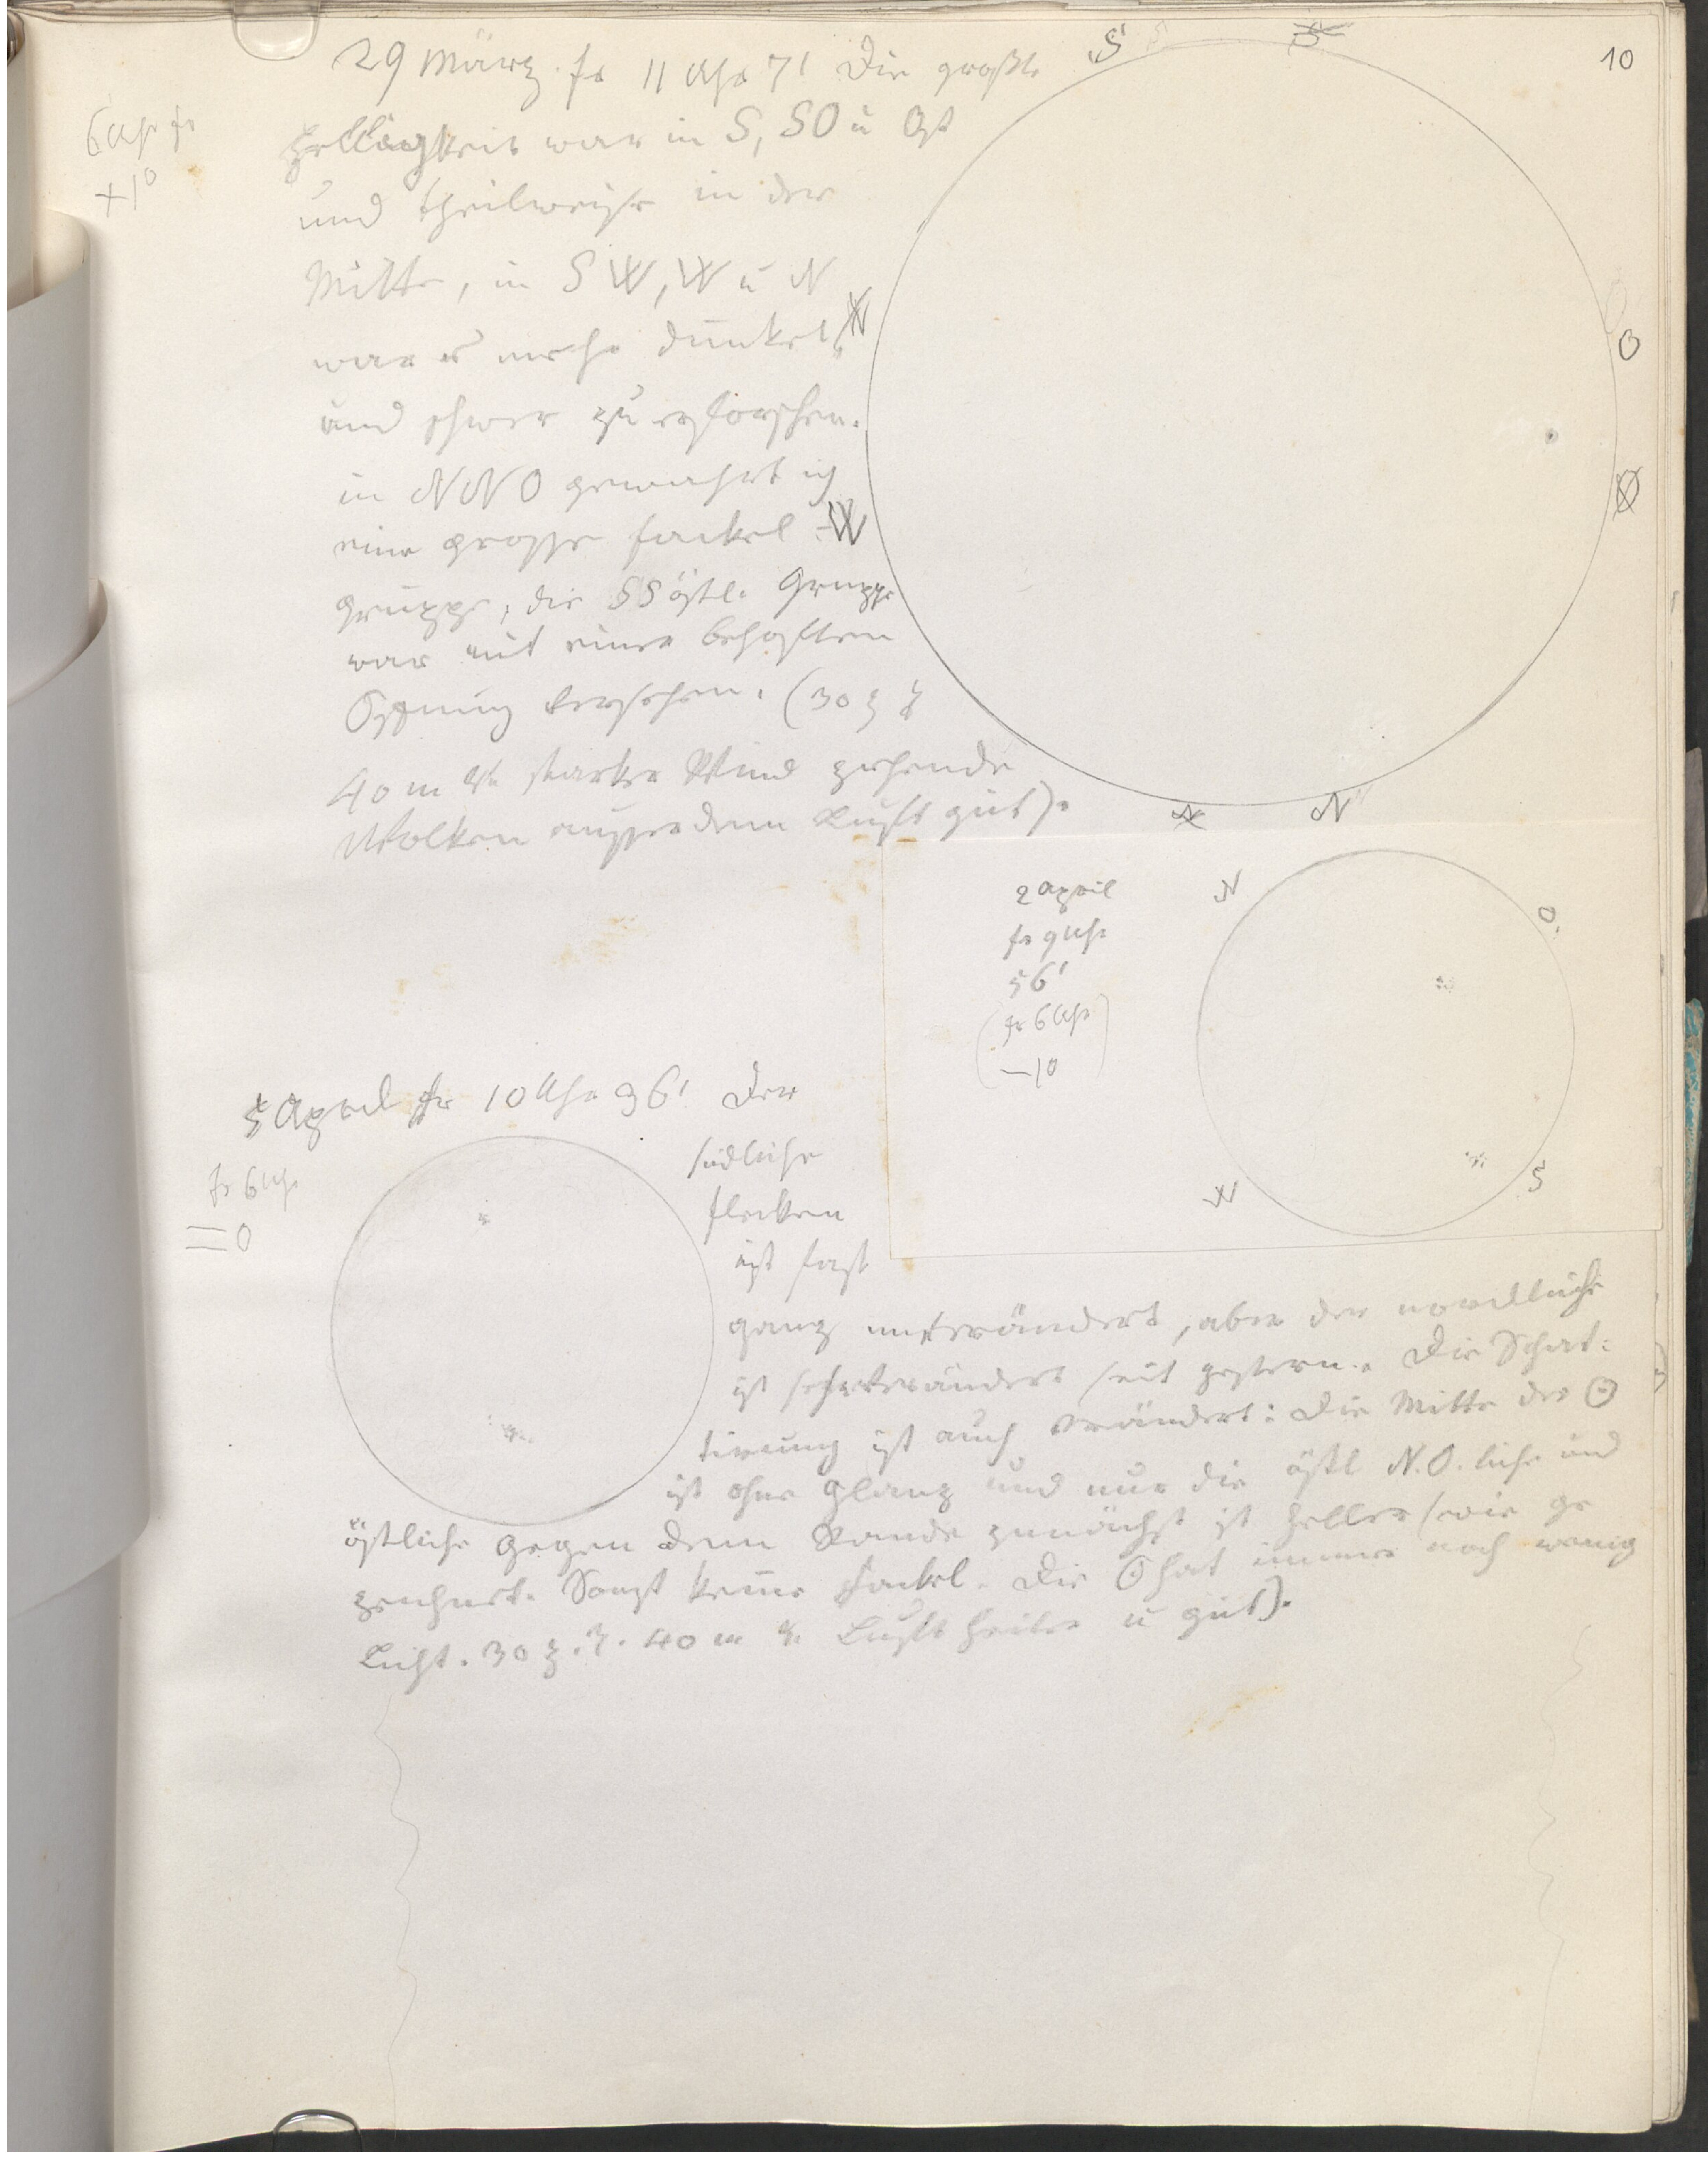
\includegraphics[width=0.5\linewidth]{./figures/gruithuisen/sample1.jpg}
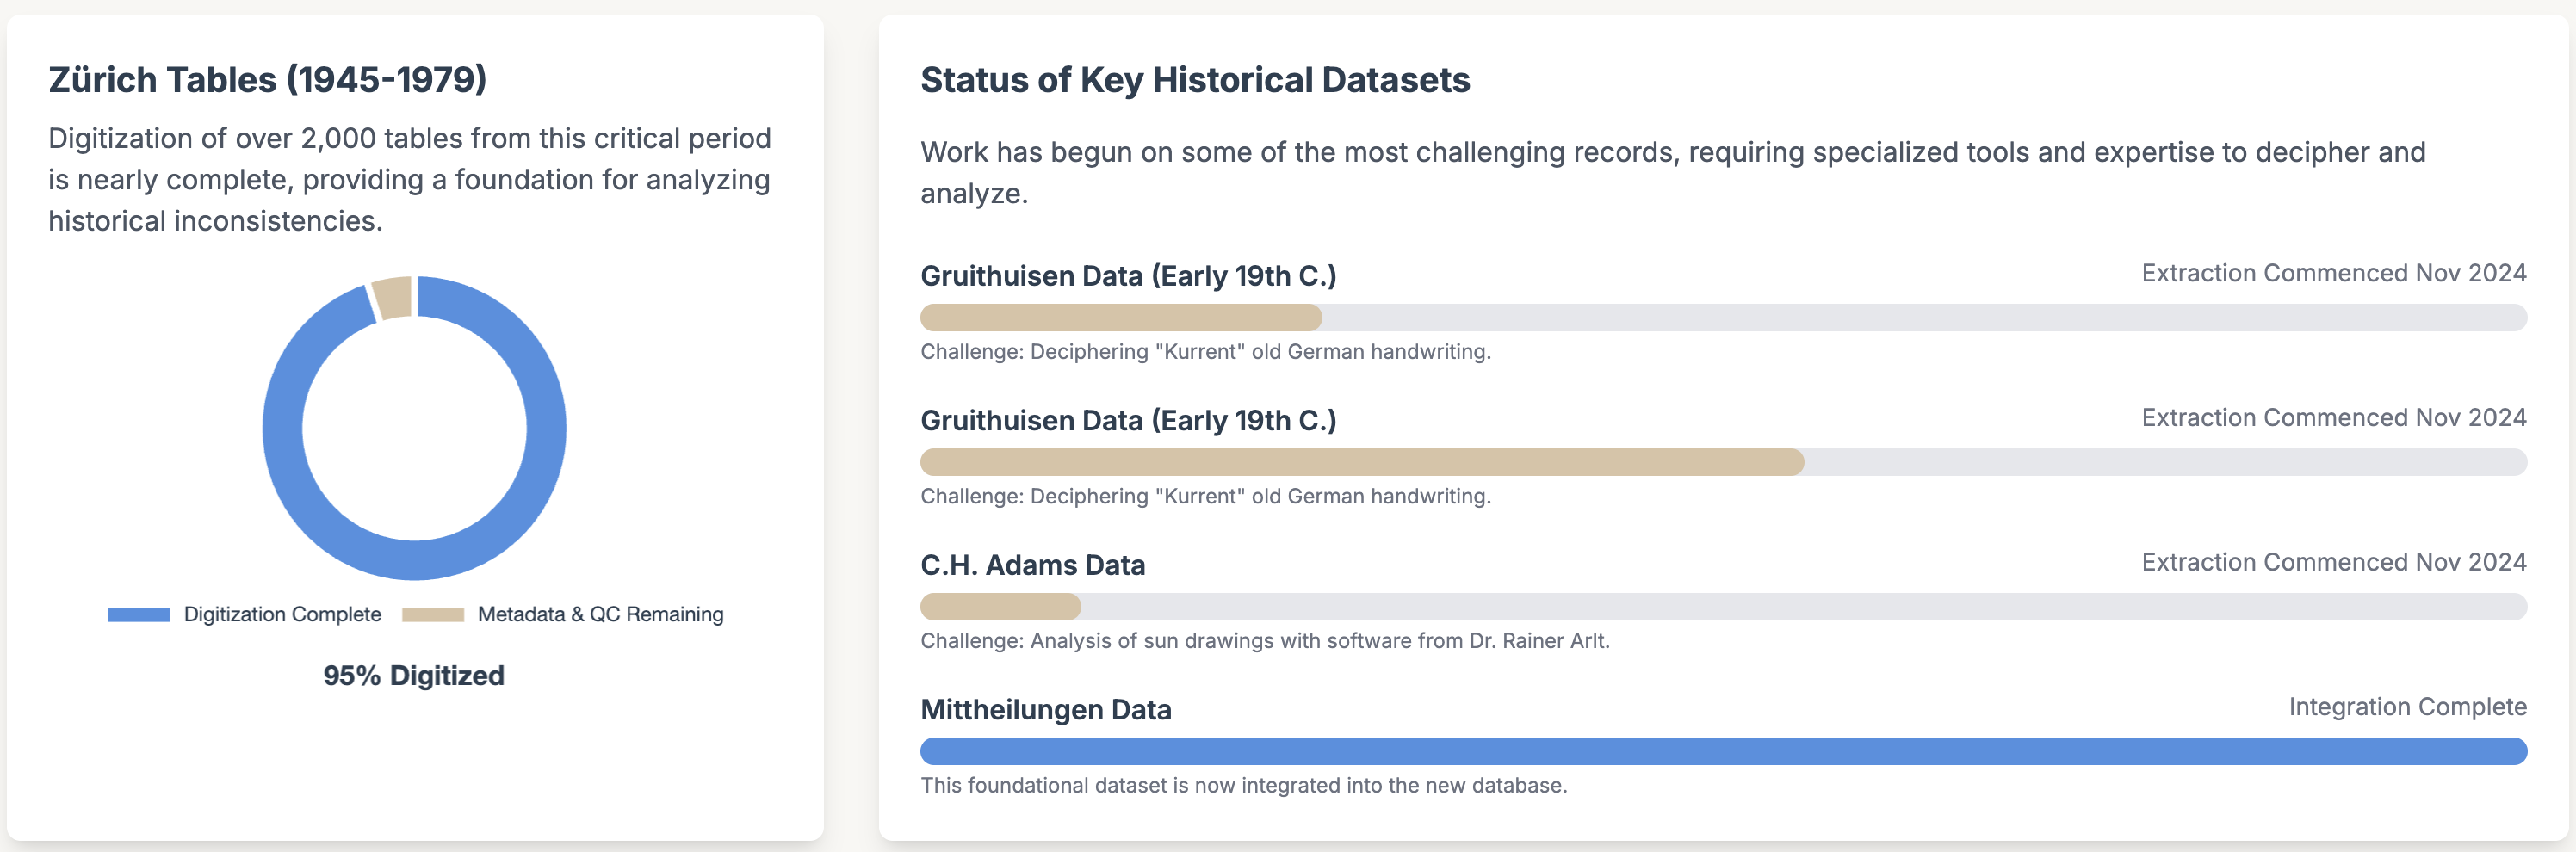
\includegraphics[width=\linewidth]{./figures/dataset_progress.png}
\end{tightblock}

\begin{tightblock}{Observer Timeline}
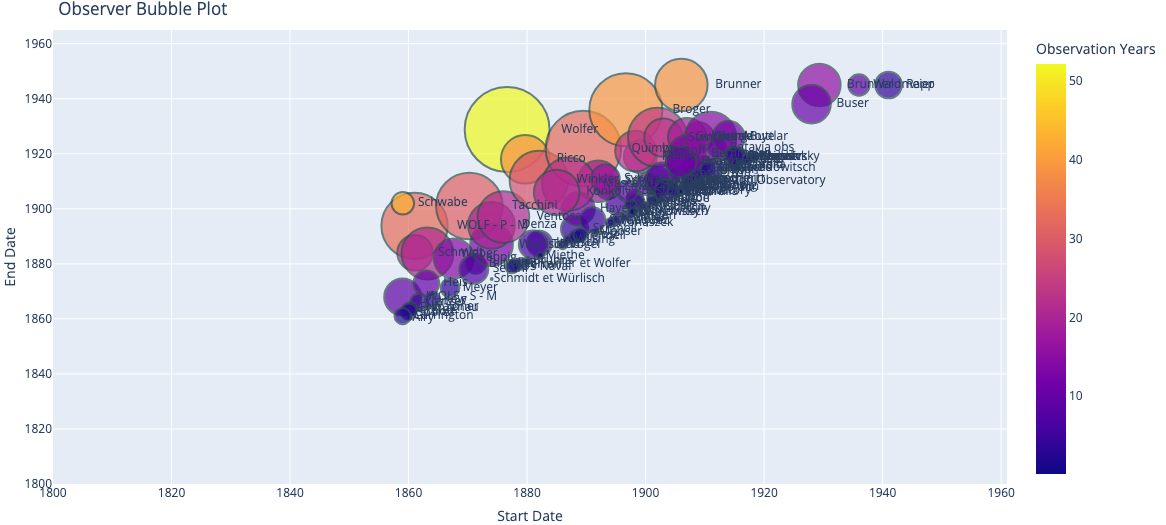
\includegraphics[width=\linewidth]{./figures/observers_bubble.png}
\scriptsize (Bubble size = total observations; color = years)
\end{tightblock}

\begin{tightblock}{Methods}
\begin{itemize}
  \item Transcription: OCR/HWR + Transkribus
  \item Normalization: unified dates, observer IDs
  \item Uncertainties: propagate errors
  \item Reproducibility: scripted pipelines
\end{itemize}
\end{tightblock}
\end{column}

% -------- COLUMN 3 --------
\begin{column}{0.32\paperwidth}
\begin{tightblock}{From Raw to ISN V3}
\begin{enumerate}
  \item Curate daily counts
  \item Calibrate observers
  \item Aggregate to monthly/yearly
  \item Compare vs. SN V2
\end{enumerate}
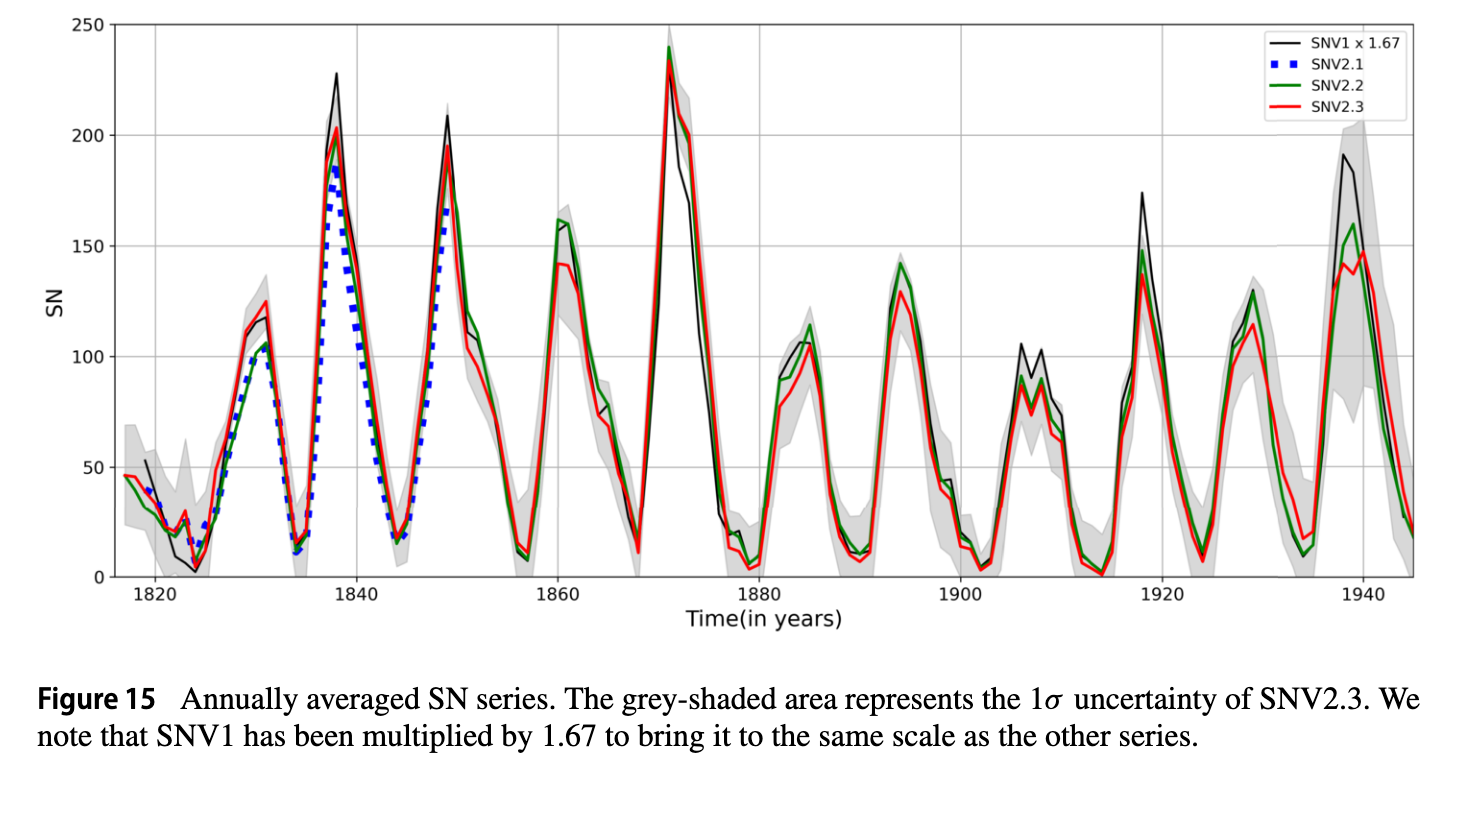
\includegraphics[width=0.9\linewidth]{./figures/comparison_panel.png}
\end{tightblock}

\begin{tightblock}{Challenges}
\begin{itemize}
  \item Handwriting (\emph{Kurrent})
  \item Heterogeneous formats
  \item Observer bias
  \item Provenance tracking
\end{itemize}
\end{tightblock}

\begin{tightblock}{Impact}
\begin{itemize}
  \item Better forecasts
  \item Long-term variability
  \item Space weather baselines
  \item Climate model inputs
\end{itemize}
\end{tightblock}

\begin{tightblock}{Outlook}
\begin{itemize}
  \item Citizen science portal
  \item Data releases + VO access
  \item Collaboration open
\end{itemize}
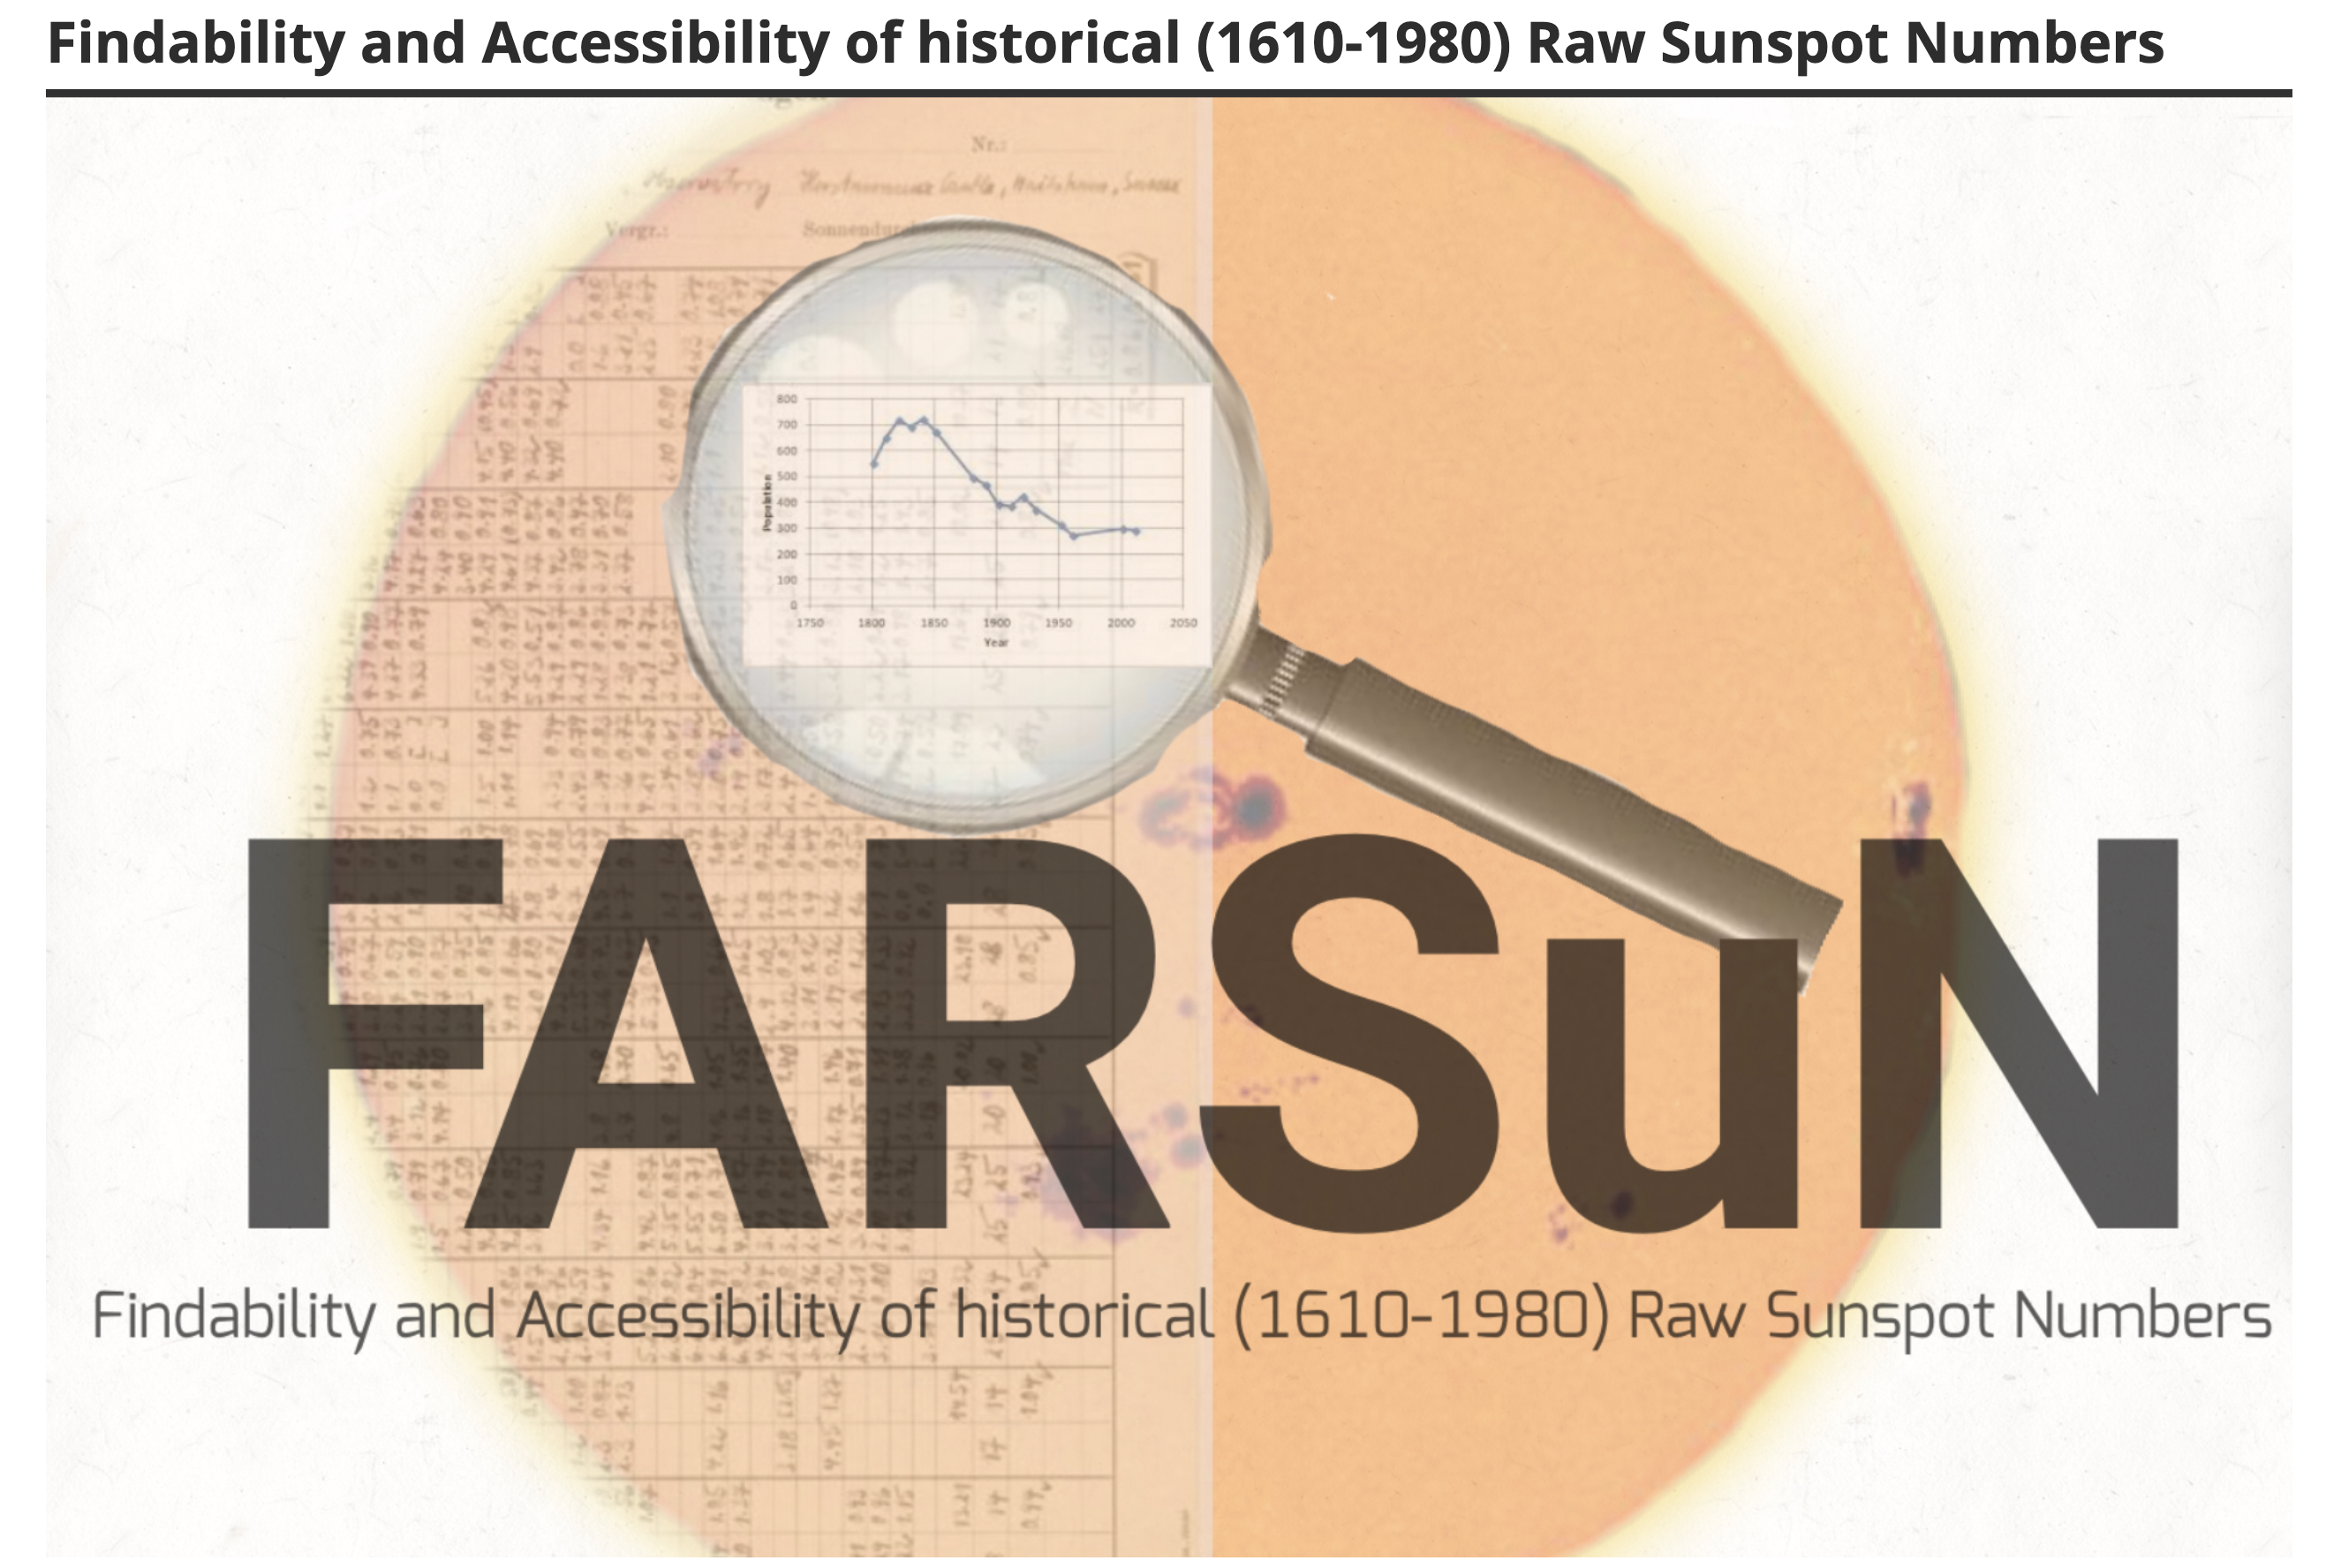
\includegraphics[width=0.8\linewidth]{./figures/ack_.png}
\end{tightblock}

\begin{tightblock}{References}
{\footnotesize \bibliography{articles}}
\end{tightblock}
\end{column}

\end{columns}
\end{frame}
\end{document}
